%!TEX root = ../doc.tex
\chapter{Concept}
\label{sec:Concept}
A working prototype of an AR system consists of two key components: Awareness regarding the environment and awareness regarding the motion of a recording camera.\\
Scanning the environment is required for a system to know what parts of the image could be enhanced by a virtual object. This prototype will focus on motion estimation, omitting surface detection.\\
Tracking the exact motion of the camera allows adjusting the position of the projected rectangle accordingly, as visualized in Figure \ref{fig:HW_concept}.
\begin{figure}[H]
    \centering
    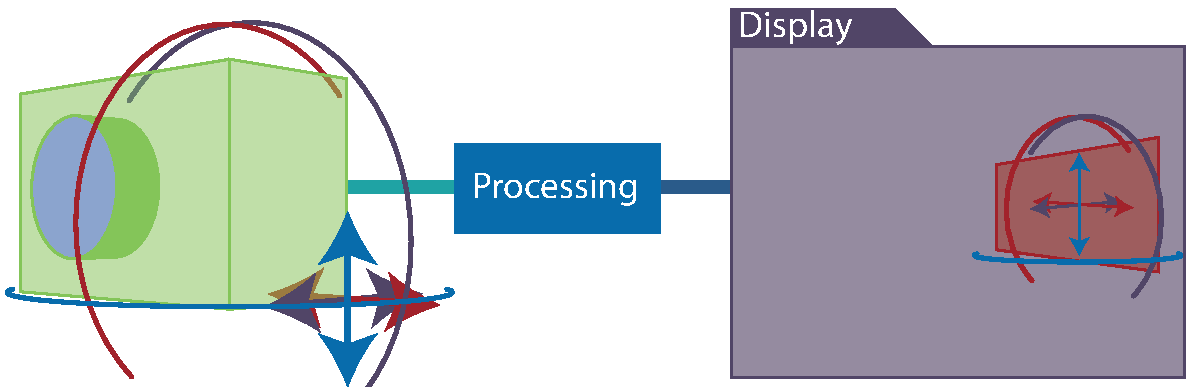
\includegraphics[width=1.0\textwidth]{images/concept_image.pdf}
    \caption{A free moving camera films the surroundings, that are displayed on the purple screen. Motion of the camera shall alter a virtual surface, projected into the display image, as if the virtual surface is stationary, despite of the motion of the camera.}
    \label{fig:HW_concept}
\end{figure}
The prototype is developed on a Nvidia Jetson Xavier AGX 8GB system with an attached accelerometer- and gyroscope-sensor, a time of flight (ToF) camera, and a Raspberry Pi Camera.\\
The three-dimensional information from the ToF camera allows extracting motion information on a frame-by-frame basis. The accelerometer complements the motion information given by the camera, especially at very fast motions. The Raspberry Pi camera acts as a viewfinder, rendered in full-size to the purple area in Figure \ref{fig:HW_concept}.\\
The projected rectangle acts as a secondary screen, allowing to display any image, the output of an additional camera or debug-images.
